%\documentclass[icelandic]{beamer}

\documentclass[icelandic,a4paper,12pt]{article}
\usepackage{beamerarticle}

\mode<presentation>
{
  \usetheme{boxes}
  % með efnisyfirliti: Szeged, Frankfurt 
  % án efnisyfirlits: Pittsburgh
  % áhugavert: CambridgeUS, Boadilla
  %\setbeamercovered{transparent} %gegnsætt
  \setbeamercovered{invisible}
  }

\usepackage[english,icelandic]{babel}
\usepackage[utf8]{inputenc}
\usepackage{t1enc}
\selectlanguage{icelandic}
\usepackage{graphicx}
\usepackage{amsmath}
\usepackage{amssymb}
\usepackage{mathrsfs}
% \newcommand{\C}{{\mathbb  C}}
% \newcommand{\Z}{{\mathbb Z}}
% \newcommand{\R}{{\mathbb  R}}
% \newcommand{\N}{{\mathbb  N}}
% \newcommand{\Q}{{\mathbb Q}}
\renewcommand{\phi}{\varphi}
\renewcommand{\epsilon}{\varepsilon}

%\usepackage{pgfpages}
% \pgfpagesuselayout{2 on 1}[a4paper,border shrink=5mm]

\def\lecturename{Stærðfræðigreining IB}
\title{\insertlecture}
\author{Benedikt Steinar Magnússon, \href{mailto:bsm@hi.is}{bsm@hi.is}}
\institute
{
  Verkfræði- og náttúruvísindasvið\\
  Háskóli Íslands
}
\subtitle{Stærðfræðigreining IB}
%\subject{\lecturename}

\mode<article>
{
	\usepackage[colorlinks=false,
	pdfauthor={Benedikt Steinar Magnusson},
	pdftitle={IB: Namsefni
	}]{hyperref}
  %\usepackage{times}
  %\usepackage{mathptmx}
  \usepackage[left=1.5cm,right=4cm,top=1.5cm,bottom=3cm]{geometry}
}

% Beamer version theme settings

%\useoutertheme[height=0pt,width=2cm,right]{sidebar}
%\usecolortheme{rose,sidebartab}
%\useinnertheme{circles}
%\usefonttheme[only large]{structurebold}

\setbeamercolor{sidebar right}{bg=black!15}
\setbeamercolor{structure}{fg=blue}
\setbeamercolor{author}{parent=structure}

\setbeamerfont{title}{series=\normalfont,size=\LARGE}
\setbeamerfont{title in sidebar}{series=\bfseries}
\setbeamerfont{author in sidebar}{series=\bfseries}
\setbeamerfont*{item}{series=}
\setbeamerfont{frametitle}{size=}
\setbeamerfont{block title}{size=\small}
\setbeamerfont{subtitle}{size=\normalsize,series=\normalfont}

\defbeamertemplate*{footline}{infolines theme}
 {
   \leavevmode%
   \hbox{%
   \begin{beamercolorbox}[wd=.333333\paperwidth,ht=2.25ex,dp=1ex,center]{author in head/foot}%
   %  \usebeamerfont{author in head/foot}\insertshortauthor~~\beamer@ifempty{\insertshortinstitute}{}{(\insertshortinstitute)}
   \end{beamercolorbox}%
   \begin{beamercolorbox}[wd=.333333\paperwidth,ht=2.25ex,dp=1ex,center]{title in head/foot}%
    % \usebeamerfont{title in head/foot}\insertshorttitle
   \end{beamercolorbox}%
   \begin{beamercolorbox}[wd=.333333\paperwidth,ht=2.25ex,dp=1ex,right]{date in head/foot}%
     %\usebeamerfont{date in head/foot}\insertshortdate{}\hspace*{2em}
     \insertshortlecture.\insertframenumber{} / \insertshortlecture.\inserttotalframenumber\hspace*{2ex} 
   \end{beamercolorbox}}%
   \vskip0pt%
 }
  


\setbeamertemplate{sidebar right}
{
  {\usebeamerfont{title in sidebar}%
    \vskip1.5em%
    \hskip3pt%
    \usebeamercolor[fg]{title in sidebar}%
    \insertshorttitle[width=2cm-6pt,center,respectlinebreaks]\par%
    \vskip1.25em%
  }%
  {%
    \hskip3pt%
    \usebeamercolor[fg]{author in sidebar}%
    \usebeamerfont{author in sidebar}%
    \insertshortauthor[width=2cm-2pt,center,respectlinebreaks]\par%
    \vskip1.25em%
  }%
  \hbox to2cm{\hss\insertlogo\hss}
  \vskip1.25em%
  \insertverticalnavigation{2cm}%
  \vfill
  \hbox to 2cm{\hfill\usebeamerfont{subsection in
      sidebar}\strut\usebeamercolor[fg]{subsection in
      sidebar}\insertshortlecture.\insertframenumber\hskip5pt}%
  \vskip3pt%
}%

\setbeamertemplate{title page}
{
  \vbox{}
  \vskip1em
  %{\huge Kapitel \insertshortlecture\par}
  {\usebeamercolor[fg]{title}\usebeamerfont{title}\inserttitle\par}%
  \ifx\insertsubtitle\@empty%
  \else%
    \vskip0.25em%
    {\usebeamerfont{subtitle}\usebeamercolor[fg]{subtitle}\insertsubtitle\par}%
  \fi%     
  \vskip1em\par
  %Vorlesung \emph{\lecturename}\ vom 
  \insertdate\par
  \vskip0pt plus1filll
  \leftskip=0pt plus1fill\insertauthor\par
  \insertinstitute\vskip1em
}

%\logo{\includegraphics[width=2cm]{beamerexample-lecture-logo.pdf}}



% Article version layout settings

\mode<article>

\makeatletter
\def\@listI{\leftmargin\leftmargini
  \parsep 0pt
  \topsep 5\p@   \@plus3\p@ \@minus5\p@
  \itemsep0pt}
\let\@listi=\@listI


\setbeamertemplate{frametitle}{\paragraph*{\insertframetitle\
    \ \small\insertframesubtitle}\ \par
}
\setbeamertemplate{frame end}{%
  \marginpar{\scriptsize\hbox to 1cm{\sffamily%
      \hfill\strut\insertshortlecture.\insertframenumber}\hrule height .2pt}}
\setlength{\marginparwidth}{1cm}
\setlength{\marginparsep}{1.5cm}

\def\@maketitle{\makechapter}

\def\makechapter{
  \newpage
  \null
  \vskip 2em%
  {%
    \parindent=0pt
    \raggedright
    \sffamily
    \vskip8pt
    %{\fontsize{36pt}{36pt}\selectfont Kapitel \insertshortlecture \par\vskip2pt}
    {\fontsize{24pt}{28pt}\selectfont \color{blue!50!black} \insertlecture\par\vskip4pt}
    {\Large\selectfont \color{blue!50!black} \insertsubtitle, \@date\par}
    \vskip10pt

    \normalsize\selectfont \@author\par\vskip1.5em
    %\hfill BLABLA
  }
  \par
  \vskip 1.5em%
}

\let\origstartsection=\@startsection
\def\@startsection#1#2#3#4#5#6{%
  \origstartsection{#1}{#2}{#3}{#4}{#5}{#6\normalfont\sffamily\color{blue!50!black}\selectfont}}

\makeatother

\mode
<all>




% Typesetting Listings

\usepackage{listings}
\lstset{language=Java}

\alt<presentation>
{\lstset{%
  basicstyle=\footnotesize\ttfamily,
  commentstyle=\slshape\color{green!50!black},
  keywordstyle=\bfseries\color{blue!50!black},
  identifierstyle=\color{blue},
  stringstyle=\color{orange},
  escapechar=\#,
  emphstyle=\color{red}}
}
{
  \lstset{%
    basicstyle=\ttfamily,
    keywordstyle=\bfseries,
    commentstyle=\itshape,
    escapechar=\#,
    emphstyle=\bfseries\color{red}
  }
}



% Common theorem-like environments

\theoremstyle{definition}
\newtheorem{exercise}[theorem]{\translate{Exercise}}




% New useful definitions:

\newbox\mytempbox
\newdimen\mytempdimen

\newcommand\includegraphicscopyright[3][]{%
  \leavevmode\vbox{\vskip3pt\raggedright\setbox\mytempbox=\hbox{\includegraphics[#1]{#2}}%
    \mytempdimen=\wd\mytempbox\box\mytempbox\par\vskip1pt%
    \fontsize{3}{3.5}\selectfont{\color{black!25}{\vbox{\hsize=\mytempdimen#3}}}\vskip3pt%
}}

\newenvironment{colortabular}[1]{\medskip\rowcolors[]{1}{blue!20}{blue!10}\tabular{#1}\rowcolor{blue!40}}{\endtabular\medskip}

\def\equad{\leavevmode\hbox{}\quad}

\newenvironment{greencolortabular}[1]
{\medskip\rowcolors[]{1}{green!50!black!20}{green!50!black!10}%
  \tabular{#1}\rowcolor{green!50!black!40}}%
{\endtabular\medskip}



\lecture[1]{2. Markgildi og samfelldni}{lecture-text}
\date{29. ágúst 2015}

\newcommand{\C}{{\mathbb  C}}
\newcommand{\Z}{{\mathbb Z}}
\newcommand{\R}{{\mathbb  R}}
\newcommand{\N}{{\mathbb  N}}
\newcommand{\Q}{{\mathbb Q}}

\begin{document}
\tableofcontents



\section{Afleiður}

\subsubsection*{Nauðsynleg undirstaða}

\subsection{Skilgreining á afleiðu}

\subsubsection{Skilgreining}
Látum $x$ vera innri punkt 
skilgreiningarsvæðis falls $f$. \emph{Afleiða falls} $f$ \emph{í punkti} $x$
er skilgreind sem 
$$f'(x)=\lim_{h\rightarrow 0}\frac{f(x+h)-f(x)}{h}.$$
Ef markgildið er til þá er sagt að fallið $f$ sé \emph{diffranlegt í
punktinum} $x$, en annars er sagt að fallið sé \emph{ekki diffranlegt í
punktinum} $x$.

\subsubsection{Dæmi} Fallið $f(x) = x^2$ er diffranlegt í sérhverjum punkti $x$. 
Það sést af því að
$$
\lim_{h\to 0^+} \frac{f(x+h)-f(x)}{h} = \lim_{h\to 0^+} \frac{(x+h)^2-x^2}{h} =
\lim_{h\to 0^+} \frac{x^2+2xh+h^2-x^2}{h}= 
\lim_{h\to 0^+} \frac{2xh+h^2}{h}= \lim_{h\to 0^+} 2x+h = 2.
$$

\subsubsection{Setning}
Ef fall $f$ er diffranlegt í punkti $c$ þá er $f$ samfellt í punktinum
$c$.

\subsubsection{Sönnun}
Skoðum markgildið $f'(x)=\lim_{h\to 0} \frac{f(c+h)-f(c)}{h}$. 
Þar sem $h\to 0$ þá verður teljarinn einnig að stefna á 0. 
Það er $\lim_{h \to 0} f(c+h)-f(c) = 0$, eða $\lim_{h \to 0} f(c+h) = f(c)$.
Þetta má einnig rita $\lim_{x \to c} f(x) = f(c)$, sem þýðir að
fallið $f$ er samfellt í $x=c$.

\subsubsection{Athugasemd}
Fall getur verið samfellt í punkti $c$ án þess að það sé
diffranlegt í $c$.

\subsubsection{Dæmi} Fallið $f(x) = |x|$ er samfellt. En það er ekki diffranlegt í 
punktinum $x=0$. \pause Það sést af því að
$$
\lim_{h\to 0^+} \frac{f(0+h)-f(0)}{h} = \lim_{h\to 0^+} \frac{|h|}{h}
= 1
$$
\pause
en
$$
\lim_{h\to 0^-} \frac{f(0+h)-f(0)}{h} = \lim_{h\to 0^-} \frac{|h|}{h}
= -1.
$$
\pause
Það er, markgildið $\lim_{h\to 0} \frac{f(0+h)-f(0)}{h}$ er ekki til.

\subsubsection{Snertill}
 Afleiðu falls $f$ í punktinum $a$ fæst með því að 
 taka sniðil í gegnum punktana $(a,f(a))$ og $(a+h,f(a+h))$, og láta
 svo $h$ stefna á $0$. 
  
 Þetta gefur hallatölu snertilsins við graf fallsins í punktinum $(a,f(a))$
 
 Snertilsins við graf fallsins er þá línan
 \begin{equation*}
	y = f'(a)(x-a) + f(a).
 \end{equation*}
 
\subsubsection{Athugasemd -- Hallatalan $\infty$ ekki leyfð}
Við leyfum ekki að $f'(a) = \infty$. \pause Samanber 
$f(x) = x^{\frac 13}$ í $a=0$,\pause
\begin{equation*}
	\lim_{h \to 0} \frac{f(0+h)-f(0)}h = 
	\lim_{h \to 0} \frac{h^{\frac 13}}h = 
	\lim_{h \to 0} h^{-\frac 23} = \infty.
\end{equation*}
\pause
Hér ætti því jafna snertilsins að vera $x=0$.
\begin{center}
 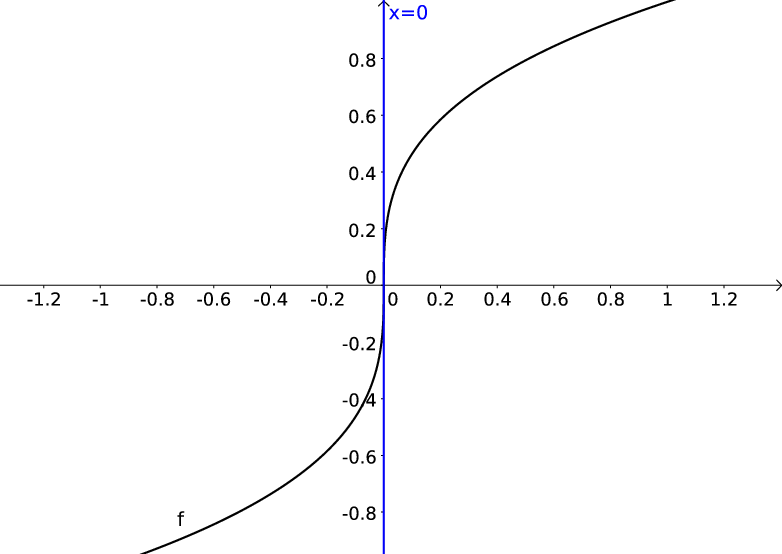
\includegraphics[width=7cm,keepaspectratio=true]{./myndir/kafli03/01_x13.png}
 % Mynd_vorpunar.eps: 277x122 pixel, 300dpi, 2.35x1.03 cm, bb=0 0 277 122
\end{center}
\pause
Viljum að snertillinn sé nálgun við graf fallsins 
fyrir $x$ nálægt $a$, lóðrétt lína er gagnslaus nálgun.


\subsection{Útvíkkun fyrir lokuð bil}
 Ef fallið $f$ er skilgreint á lokuðu bili þá getum við skilgreint  afleiðuna í endapunktunum
 með því að taka markgildi frá hægri/vinstri eftir því sem við á.
 
 \subsubsection{Skilgreining}
\begin{enumerate}[(i)]
\item \emph{Hægri afleiða falls} $f$ \emph{í punkti} $x$ er skilgreind sem 
$$
	f_+'(x)=\lim_{h\rightarrow 0^+}\frac{f(x+h)-f(x)}{h}.
$$
\item \emph{Vinstri afleiða falls} $f$ \emph{í punkti} $x$ er skilgreind sem 
$$
	f_-'(x)=\lim_{h\rightarrow 0^-}\frac{f(x+h)-f(x)}{h}.
$$
\end{enumerate}

\subsubsection{Setning}
Ef $x$ er innri punktur í skilgreiningarsvæði fallsins $f$ þá er $f$ diffranlegt
í $x$ þá og því að eins
$$
	f_+'(x)=\lim_{h\rightarrow 0^+}\frac{f(x+h)-f(x)}{h}
=	f_-'(x)=\lim_{h\rightarrow 0^-}\frac{f(x+h)-f(x)}{h},
$$
og þá er $f'(x)$ jafnt og markgildin hér fyrir ofan.

\subsubsection{Skilgreining}
Látum $f$ vera fall með skilgreiningarsvæði
$A$.  Gerum ráð fyrir að $A$ sé sammengi endanlega margra bila.  Við
segjum að fallið $f$ sé \emph{diffranlegt} ef það er diffranlegt í öllum 
innri punktum $A$ og diffranlegt frá vinstri/hægri í jaðarpunktum $A$ 
eftir því sem við á.

\subsection{Athugasemd -- Ritháttur}
Afleiða falls $f$ er ýmist táknuð með
$$
  f', \qquad \frac {df}{dx}, \qquad D_x f \qquad \text{eða } Df.
$$
Ef við skrifum $y=f(x)$ þá má einnig tákna hana með 
$$
  y', \qquad \frac {dy}{dx}, \qquad D_x y \qquad \text{eða } Dy.
$$

\subsubsection{Dæmi}
Fallið $f(x) = \sqrt{x}$, $f:[0,\infty[\to \R$ er diffranlegt á 
menginu $]0,\infty[$ og afleiðan er gefin
með $f'(x) = \frac 1{2\sqrt{x}} = \frac 12 x^{-1/2}$ þar. Hins vegar er $f$ 
ekki diffranlegt í $x=0$ þrátt fyrir að fallgildið sé vel skilgreint (og fallið samfellt 
frá hægri) þar.

Ef $x>0$ þá fæst
\begin{align*}
  \lim_{h\to 0} \frac{\sqrt{x+h}-\sqrt{x}}h &= 
  \lim_{h\to 0} \frac{(\sqrt{x+h}-\sqrt{x})(\sqrt{x+h}+\sqrt{x})}{h(\sqrt{x+h}+\sqrt{x})}\\ 
  &= \lim_{h\to 0} \frac{\sqrt{x+h}^2-\sqrt{x}^2}{h(\sqrt{x+h}+\sqrt{x})}\\
  &= \lim_{h\to 0} \frac{x+h-x}{h(\sqrt{x+h}+\sqrt{x})}\\
  &= \lim_{h\to 0} \frac{1}{\sqrt{x+h}+\sqrt{x}} = \frac{1}{2\sqrt{x}},
\end{align*}
sem segir okkur að $f'(x) = \frac 12 x^{-1/2}$.

Í vinstri endapunkti skilgreingarsvæðisins, $x=0$, þá fæst hins vegar
\begin{align*}
  \lim_{h\to 0^+} \frac{\sqrt{h}-\sqrt{0}}h &= 
  \lim_{h\to 0^+} \frac{\sqrt{h}}h\\
  &= \lim_{h\to 0^+} \frac{1}{\sqrt{h}} = \infty,
\end{align*}
sem sýnir að fallið er ekki diffranlegt frá hægri í $x=0$.

\subsection{Reiknireglur}
\subsubsection{Setning}\label{setn:diffreglur}
Látum $f$ og $g$ vera föll sem eru diffranleg í punkti $x$.  Þá eru
föllin $f+g,\ f-g, kf$ (þar sem $k$ er fasti) og $fg$
diffranleg í punktinum $x$, og ef $g(x)\neq 0$ þá eru föllin
$1/g$ og $f/g$ líka diffranleg í $x$.
\pause

Eftirfarandi formúlur gilda um afleiður fallanna sem talin eru upp hér að
framan: 
\begin{enumerate}[(i)]
\item $(f+g)'(x)=f'(x)+g'(x)$ \pause
\item $(f-g)'(x)=f'(x)-g'(x)$\pause
\item $(kf)'(x)=kf'(x)$, þar sem $k$ er fasti\pause
\item $(fg)'(x)=f'(x)g(x)+f(x)g'(x)$\pause
\item $\displaystyle\Bigg(\frac{1}{g}\Bigg)'(x)=\frac{-g'(x)}{g(x)^2}$,  ef
  $g(x)\neq 0$\pause
\item $\displaystyle\Bigg(\frac{f}{g}\Bigg)'(x)=
\frac{f'(x)g(x)-f(x)g'(x)}{g(x)^2}$, ef
  $g(x)\neq 0$
\end{enumerate}

\subsubsection{Nokkrar afleiður}
\begin{enumerate}[(i)]
\item $\frac{d}{dx} c \pause=  \lim_{h\to 0} \frac{c-c}h = 0$
\item $\frac{d}{dx} x \pause=  \lim_{h\to 0} \frac{x+h-x}h = 1$
\item $\frac{d}{dx} x^2 \pause= \lim_{h\to 0} \frac{x^2+2xh+h^2-x^2}h
= \lim_{h\to 0} \frac{2xh + h^2}h \pause= \lim_{h\to 0} 2x+h= 2x$
\end{enumerate}
\pause

\subsubsection{Setning}\label{setn:diff_xn}
\begin{equation*}
	\frac{d}{dx} x^n = n x^{n-1}
\end{equation*}\pause
{\bf Sönnun:} Sýnum þetta með þrepun.\pause 
Tilfellið $n=1$ er afgreitt
hér að ofan. \pause Gerum ráð fyrir að niðurstaðan gildi fyrir $n$ og
sýnum að þá gildi hún einnig fyrir $n+1$,\pause
\begin{equation*}
	\frac{d}{dx} x^{n+1} =\pause \frac{d}{dx} (x\cdot x^n) = \pause
	\left(\frac{d}{dx} x\right) x^n + x\frac{d}{dx} x^n\pause
	= x^n + x\, 
	\underbrace{n\, x^{n-1}}_\text{þ.f.} \pause
	= (n+1) x^n.
\end{equation*}


\subsubsection{Afleiður margliða}
Með því að nota setningarnar að ofan þá eigum við ekki í neinum vandræðum með að 
diffra margliður. Setning \ref{setn:diffreglur} (i) segir að við getum diffrað 
hvern lið fyrir sig, liður (iii) í sömu setningu segir að við getum tekið fastana 
fram fyrir afleiðuna og loks segir setning \ref{setn:diff_xn} hvernig við 
diffrum $x^n$.

\subsubsection{Dæmi}
Finnum afleiðu margliðunnar $p(x) = 4x^3-2x + 5$. Nú er 
\begin{align*}
\frac{d}{dx} p(x) 
&= \frac{d}{dx}4x^3 - \frac{d}{dx}2x + \frac{d}{dx}5 \\
&= 4\frac{d}{dx}x^3 -2\frac{d}{dx}x + \frac{d}{dx}5 =
4\cdot 3x^2 -2\cdot 1 + 0 = 12x^2-2
\end{align*}

\subsection{Hærri afleiður}
\subsubsection{Skilgreining}  
Látum $f$ vera fall.  Afleiðan $f'$ er fall
sem skilgreint er í öllum punktum þar sem $f$ er diffranlegt.  

\pause

Ef fallið $f'$ er diffranlegt í punkti $x$ þá er afleiða $f'$ í
punktinum $x$ táknuð með $f''(x)$ og kölluð \emph{önnur afleiða} $f$ 
í punktinum $x$.  \pause
Líta má á aðra afleiðu $f$ sem fall $f''$ sem 
er skilgreint í öllum punktum þar sem $f'$ er diffranlegt.

\pause

Almennt má skilgreina $n$\emph{-tu afleiðu} $f$, táknaða með $f^{(n)}$, 
þannig að í þeim punktum $x$ þar sem fallið $f^{(n-1)}$ er diffranlegt 
þá er $f^{(n)}(x)=\frac{d}{dx}f^{(n-1)}(x)$.  
 

\subsubsection{Dæmi}
Ef $f(x)  = 3x^2$, þá er $f'(x) = 3\frac{d}{dx}x^2 = 3\cdot 2x = 6x$ og 
$f''(x) = 6 \frac{d}{dx} x = 6$.

%\subsection{Ritháttur fyrir afleiður}
\subsubsection{Ritháttur}   
Ritum $y=f(x)$.  
\begin{equation*}
y'= f'(x)=\frac{d}{dx}f(x)=D_xf(x)\ =\ D_x y= \frac{dy}{dx}
\end{equation*}\pause
\begin{align*}
y'' &=
f''(x)=\frac{d}{dx}f'(x)=\frac{d}{dx}\frac{d}{dx}f(x)\\
&= D^2_xf(x)= D^2_x y=\frac{d^2}{dx^2}f(x)=\frac{d^2 y}{dx^2}
\end{align*}\pause
\begin{align*}
y^{(n)} &= f^{(n)}(x)=\frac{d}{dx}f^{(n-1)}(x)=
\frac{d}{dx}\Big(\frac{d^{n-1}}{dx^{n-1}}f(x)\Big) \\
&=D^n_xf(x)\ =\ D^n_x y
=\frac{d^n}{dx^n}f(x)
= \frac{d^n y}{dx^n}.
\end{align*}

\subsubsection{Athugasemd}
Venja er að rita $f'''$ til að tákna þriðju afleiðu $f$ en afar sjaldgæft
að $f''''$ sé notað til að tákna fjórðu afleiðu $f$ og mun algengara
að nota $f^{(4)}$.  

\subsection{Útgildi}
 \subsubsection{Skilgreining}
 Við segjum að fall $f$ hafi \emph{staðbundið hágildi í punktinum} $x_0$
 ef til er bil $(a,b)$ umhverfis $x_0$, sem er þannig að 
 \begin{equation*}
	f(x) \leq f(x_0), \quad \text{ fyrir öll } x \in (a,b)
 \end{equation*}
 
 \pause
 
 Við segjum að fall $f$ hafi \emph{staðbundið lággildi í punktinum} $x_0$
 ef til er bil $(a,b)$ umhverfis $x_0$, sem er þannig að 
 \begin{equation*}
	f(x) \geq f(x_0), \quad \text{ fyrir öll } x \in (a,b)
 \end{equation*}
 
 \pause
 
 Tölum um að fallið $f$ hafi \emph{staðbundið útgildi í punktinum} $x_0$
 ef það hefur staðbundið hágildi eða staðbundið lággildi þar.
 
%\subsection{Afleiður í útgildum}
\subsubsection{Setning}\label{setn:diffutgildi}
Ef fallið $f$ hefur staðbundið útgildi í punktinum $x_0$ \pause
og er diffranlegt þá er $f'(x_0)=0$.

\subsubsection{Athugasemd}
Þó að $f'(a)=0$ þá er ekki víst að $a$ sé útgildi.

Til dæmis þá hefur fallið $f(x) = x^3$ ekkert staðbundið útgildi
en $f'(x) = 3x^2$, þ.e.~$f'(0) = 0$.
 
\subsubsection{Sönnun á Setningu \ref{setn:diffutgildi}}
Gerum ráð fyrir að $f$ hafi staðbundið hágildi í punktinum $x_0$. \\\pause
Þá er $f(x_0)-f(x)\geq 0$ ef $x<x_0$, þ.e.~$\frac{f(x_0)-f(x)}{x_0-x}\geq 0$
ef $x<x_0$. \\\pause 
Þetta þýðir að 
 \begin{equation}
	\lim_{x \to x_0^-} = \frac{f(x_0) - f(x)}{x_0-x} \geq 0.
	\label{vinstri}
 \end{equation}
 
\pause

Eins þá er $f(x_0)-f(x)\geq 0$ ef $x_0<x$, 
þ.e.~$\frac{f(x_0)-f(x)}{x_0-x} \leq 0$ ef $x_0 < x$. \pause 
Þetta þýðir að 
 \begin{equation}
	\lim_{x \to x_0^+} = \frac{f(x_0) - f(x)}{x_0-x} \leq 0.
	\label{haegri}
 \end{equation}
 
 \pause
 
 Við vitum að markgildið $\lim_{x\to x_0} \frac{f(x_0)-f(x)}{x_0-x}$ er
 til þar sem fallið er diffranlegt, það þýðir að markgildin frá hægri og
 vinstri eru þau sömu. \pause
 Eina leiðin til þess að það samræmist 
 (\ref{vinstri}) og (\ref{haegri}) er að 
 \begin{equation*}
	f'(x_0) = \lim_{x\to x_0} \frac{f(x_0)-f(x)}{x_0-x} = 0.
 \end{equation*}

%% Keðjureglan
% Mótivasjón
% Setning/sönnun
%% Hornaföll

\subsection{Keðjureglan}
\subsubsection{Setning}
Gerum ráð fyrir að $f$ og $g$ séu föll þannig að $g$ er diffranlegt í 
$x$ og  $f$ er diffranlegt í $g(x)$. Þá er samskeytingin $f\circ g$
diffranleg í $x$ og 
\begin{equation*}
	(f\circ g)'(x) = f'(g(x))\cdot g'(x).
\end{equation*}

\subsection{Hornaföll og afleiður þeirra}
 \subsubsection{Setning}
 \begin{enumerate}[(i)]
 \item $\displaystyle\lim_{x\rightarrow 0}\frac{\sin x}{x}=1$
 \pause
\item $\displaystyle\lim_{x\rightarrow 0}\frac{\cos x-1}{x}=0$
\pause
\item $\displaystyle\frac{d}{dx}\sin x=\cos x$
\pause
\item $\displaystyle\frac{d}{dx}\cos x=-\sin x$
\pause
 \item $\displaystyle\frac{d}{dx}\tan x=\frac{1}{\cos^2 x}=1+\tan^2 x$
\end{enumerate}
 
\subsection{Meðalgildissetningin}
\subsubsection{Setning Rolle}    
Látum $g:[a,b]\rightarrow\R$ vera samfellt fall.  Gerum ráð fyrir að $g$ sé diffranlegt í öllum
punktum í bilinu $(a,b)$. \pause Ef $g(a)=g(b)$ þá er til punktur $c$ á bilinu $(a,b)$ þannig að $g'(c)=0$.  
\subsubsection{Sönnun}
	Ef $g(x)=c$ er fasti, þá er $g'(x)=0$. \pause
	Ef hins vegar $g$ er ekki fasti þá er til $x \in (a,b)$ þannig
	að $g(x)\neq 0$, gerum ráð fyrir að $g(x)>0$\pause
	(tilfellið ef $g(x)<0$ gengur nánast eins fyrir sig).\pause
	Samkvæmt Há- og lággildislögmálinu (Setning 4.6) þá er tekur
	fallið $g$ sitt hæsta gildi í punkti $c$ á bilinu $[a,b]$.\pause
	Þar sem $g(c)\geq g(x) > 0 = g(a) = g(b)$ þá getur $c$ hvorki
	verið $a$ né $b$. 
	
\subsubsection{Meðalgildissetningin}   
Látum $f:[a,b]\rightarrow\R$ vera samfellt fall.  Gerum ráð fyrir að $f$ sé diffranlegt í öllum
punktum í bilinu $(a,b)$.  Þá er til punktur $c$ í bilinu $(a,b)$ þannig að
$$\frac{f(b)-f(a)}{b-a}=f'(c).$$

\subsubsection{Með öðrum orðum}
Á einhverjum punkti á bilinu er stundarbreytingin jöfn meðalbreytingunni yfir allt bilið.

\subsubsection{Alhæfða meðalgildissetningin}  Gerum ráð fyrir að föllin $f$ og
$g$ séu samfelld á lokaða bilinu $[a,b]$ og diffranleg á opna bilinu $(a,b)$.  Gerum auk
þess ráð fyrir að fyrir allar tölur $x$ í $(a,b)$ sé $g'(x)\neq 0$.  Þá er til
tala $c\in (a,b)$ þannig að $$\frac{f(b)-f(a)}{g(b)-g(a)}=\frac{f'(c)}{g'(c)}.$$

\subsection{Vaxandi og minnkandi föll}
\subsubsection{Skilgreining}
Fall $f$ er \emph{vaxandi} (nondecreasing) á bili $(a,b)$ ef um alla punkta
$x_1$ og $x_2$ á $(a,b)$ þannig að $x_1 < x_2$, þá er\vspace{-0.1in}
\begin{equation*}
	f(x_1) \leq f(x_2).
\end{equation*}

Fall $f$ er \emph{stranglega vaxandi} (increasing) á bili $(a,b)$ ef um alla punkta
$x_1$ og $x_2$ á $(a,b)$ þannig að $x_1 < x_2$, þá er\vspace{-0.1in}
\begin{equation*}
	f(x_1) < f(x_2).
\end{equation*}

Fall $f$ er \emph{minnkandi} (nonincreasing) á bili $(a,b)$ ef um alla punkta
$x_1$ og $x_2$ á $(a,b)$ þannig að $x_1 < x_2$, þá er\vspace{-0.1in}
\begin{equation*}
	f(x_1) \geq f(x_2).
\end{equation*}
	
Fall $f$ er \emph{stranglega minnkandi} (decreasing) á bili $(a,b)$ ef um alla punkta
$x_1$ og $x_2$ á $(a,b)$ þannig að $x_1 < x_2$, þá er\vspace{-0.1in}
\begin{equation*}
	f(x_1) > f(x_2).
\end{equation*}

\subsubsection{Setning}
Látum $f$ vera diffranlegt fall. Þá er $f$ vaxandi þá og því aðeins að $f' \geq 0$.

\subsubsection{Setning}
Látum $f$ vera diffranlegt fall. Þá er $f$ minnkandi þá og því aðeins að $f' \leq 0$.

\subsubsection{Setning} 
Látum $f$ vera diffranlegt fall. Ef $f'>0$ þá er $f$ stranglega vaxandi.

\subsubsection{Setning}
Látum $f$ vera diffranlegt fall. Ef $f'<0$ þá er $f$ stranglega minnkandi.

\subsubsection{Athugasemd} 
Diffranlegt fall getur verið stranglega vaxandi/minnkandi án þess að afleiðan
sé alls staðar 0. T.d.~er afleiða $f(x)=x^3$ jöfn 0 í $x=0$ en fallið er 
stranglega vaxandi á öllum rauntalnaásnum.

\subsubsection{Afleiður fastafalla}
Við vitum að ef $f$ er fasti ($f(x)=c$) þá er $f'(x)=0$ 
fyrir öll $x$ (Dæmi 5.6). 

Nú fáum við einnig eftirfarandi út úr Setningum 7.5 og 7.6.

\subsubsection{Fylgisetning}
Ef $f$ er diffranlegt fall á bili $I$ sem er þannig að $f'(x) = 0$
á $I$, þá er $f$ fasti, þ.e.~$f(x) = c$ fyrir öll $x\in I$.

\subsection{Fólgin diffrun}
\subsubsection{Dæmi}
  Jafna hrings með geisla 1 er $x^2+y^2=1$. Við vitum að hægt er
að skrifa efri og neðri helminga hans sem föll af $y$, annars
vegar $y=\sqrt{1-x^2}$ og hins vegar $y=-\sqrt{1-x^2}$.
\pause
Ef við viljum finna snertil við hringinn getum við notað þessi föll. 
\pause
En þar sem við vitum að hægt er að skrifa $y$ sem fall af $x$ þá
getum við einnig diffrað jöfnu hringsins beint með aðstoð keðjureglunnar,
\begin{eqnarray*}
\frac{d}{dx}(x^2+y^2) &=& \frac{d}{dx} 0 \\
 	2x + 2y\frac{dy}{dx} &=& 0\\
	y\frac{dy}{dx} &=& -x\\
	\frac{dy}{dx} &=& -\frac xy.
\end{eqnarray*}
\begin{center}
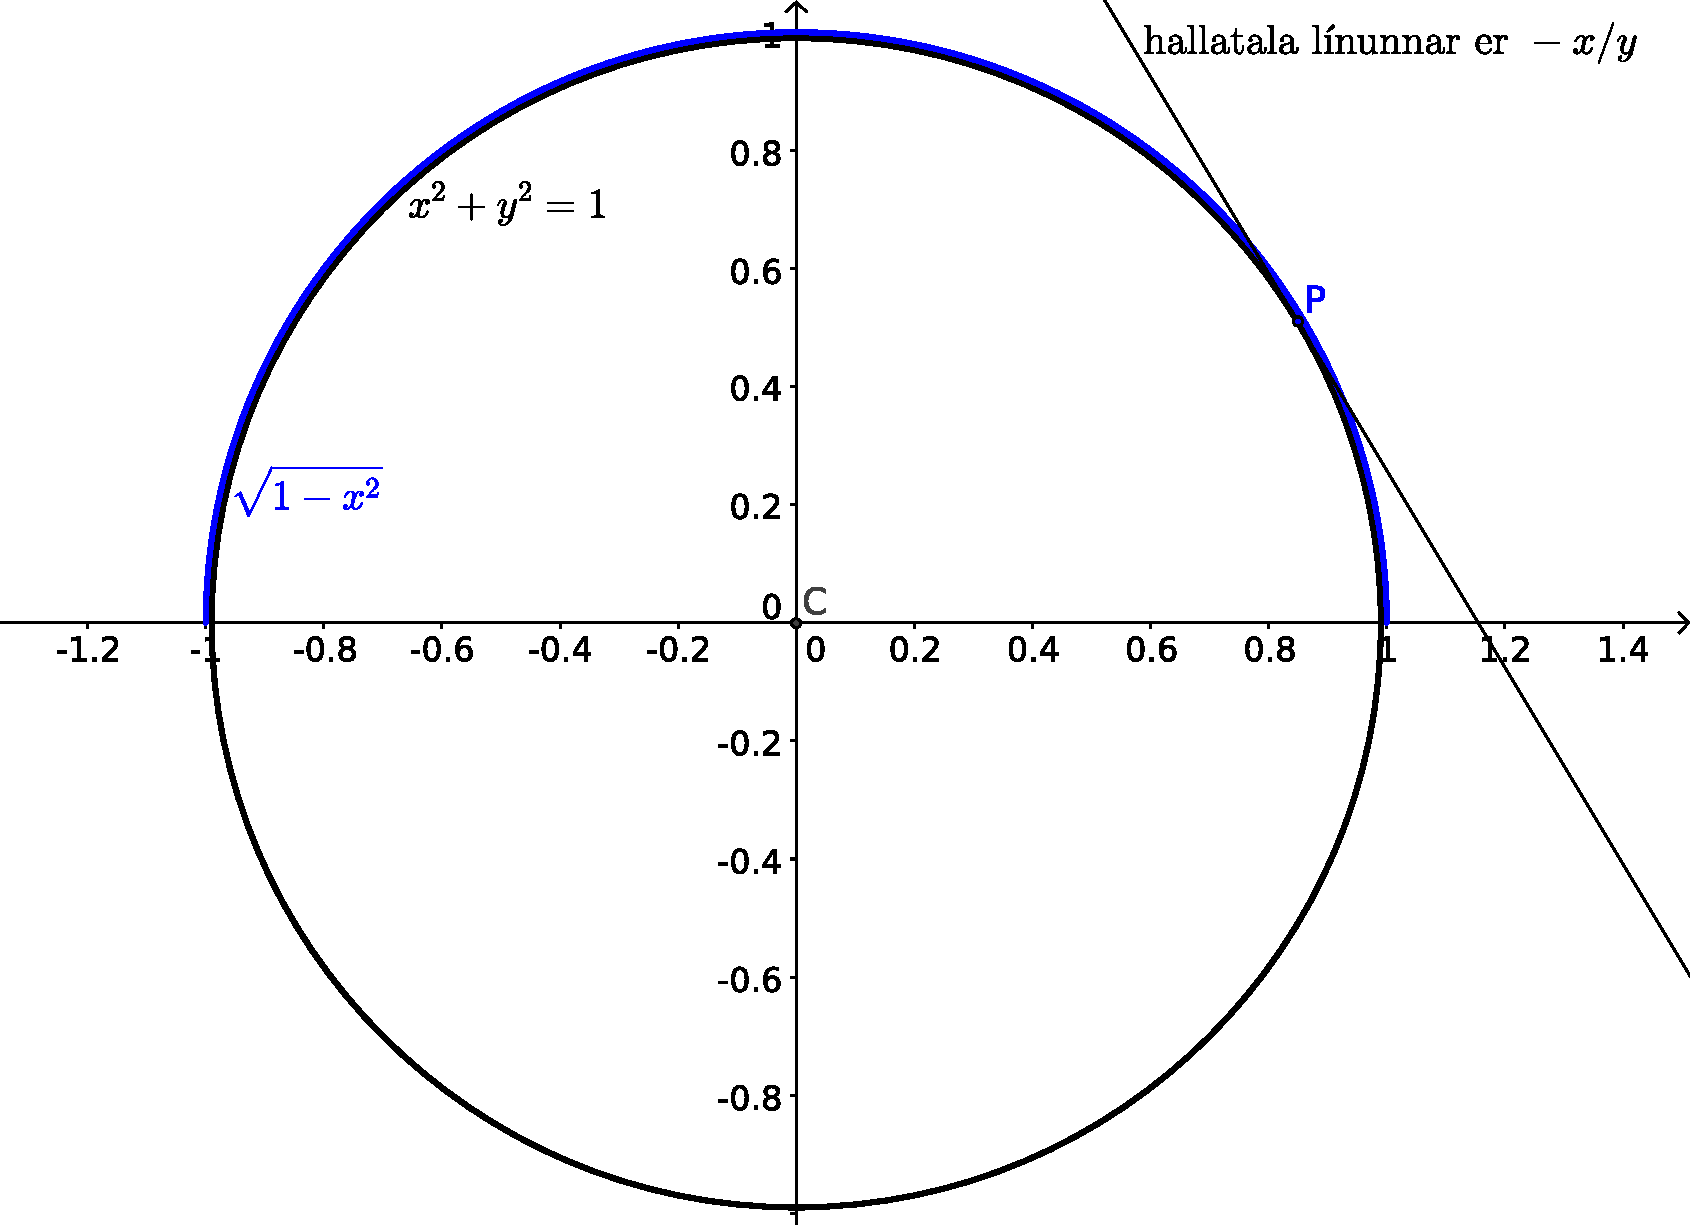
\includegraphics[width=10cm,keepaspectratio=true]{./myndir/IB11-f08_hringur-eps-converted-to.pdf}
\end{center}

\subsubsection{Setning}
Látum feril vera gefinn með $F(x,y) =0$, þar sem $F$ er diffranlegt
í bæði $x$ og $y$. Í punktum þar sem ferillinn er ekki lóðréttur
(þ.e.~$\frac{d}{dy}F \neq 0$) þá er hægt að skrifa $y$ sem fall af 
$x$ og þá fæst af keðjureglunni að 
\begin{equation*}
 \frac{d}{dx} F(x,y) + \frac{d}{dy}F(x,y) \frac{dy}{dx} = 0,
\end{equation*}
þ.e.
\begin{equation*}
\frac{dy}{dx} = -\frac{\frac{d}{dx} F(x,y)}{\frac{d}{dy} F(x,y)}.
\end{equation*}

\subsubsection{Með öðrum orðum}
Það kemur á sama stað niður að einangra $y=f(x)$, ef það er mögulegt, 
og finna $y'$ með því að diffra, eins og að diffra $F(x,y)=0$ og einangra svo 
$y'=\frac{dy}{dx}$.

\subsubsection{Vinnulag}
\begin{itemize}
\item[(i)] Diffrum beggja vegna jöfnuna með tilliti til $x$, og lítum á $y$
sem fall af $x$ sem við diffrum með aðstoð keðjureglunnar 
(og gleymum ekki $y'$)
\item[(ii)] Einangrum $y'$
\item[(iii)] Skiptum $y$ fyrir $f(x)$.
\end{itemize}

\subsubsection{Setning -- Hagnýting á fólginni diffrun}
Ef $n$ og $m$ eru heilar tölur þá er
\begin{equation*}
 \frac{d}{dx} x^{\frac nm} = \frac nm x^{\frac nm -1}.
\end{equation*}

\subsection{Andhverf föll}
\subsubsection{Skilgreining}  \emph{Skilgreiningarsvæði} falls $f$ (e.~domain) er mengi allra 
talna $x$ þannig að $f(x)$ er skilgreint.

\subsubsection{Skilgreining} 
Við segjum að fallið $f$ sé \emph{eintækt} (e.~one-to-one, injective)
ef fyrir allar tölur $x_1$ og $x_2$ úr skilgreiningarsvæði $f$ gildir
að ef $x_1\neq x_2$ þá er $f(x_1)\neq f(x_2)$. \pause
(Ólík stök varpast í ólík stök.)  \pause
Þetta má líka orða þannig að fallið $f$ er eintækt ef
alltaf þegar $f(x_1)=f(x_2)$ má álykta að $x_1=x_2$.


\subsubsection{Skilgreining}  Látum $f$ vera fall með skilgreiningarsvæði
$D$.  \emph{Myndmengi} $f$ (e.~range) er skilgreint sem mengið 
$$f(D)=\{f(x)\mid x\in D\}.$$
\pause
Myndmengið er mengi allra mögulegra útkoma úr $f$.

\subsubsection{Skilgreining og setning}
Látum $f$ vera fall sem skilgreint er á mengi $D$.  Gerum ráð fyrir að
$f$ sé eintækt.  Þá er til fall $f^{-1}$ sem er skilgreint á menginu
$f(D)$ þannig að $$y=f(x)\qquad\mbox{þá og því aðeins að}\qquad x=f^{-1}(y).$$
Fallið $f^{-1}$ kallast \emph{andhverfa} $f$.

\subsubsection{Setning}  
Fall sem er strangt vaxandi eða strangt minnkandi er eintækt og á sér því andhverfu.

\subsubsection{Eiginleikar}
\begin{itemize}
\item[(i)]  $y=f^{-1}(x)$ þá og því aðeins að $x=f(y)$.
\pause
\item[(ii)]  Skilgreingarsvæði $f$ er myndmengi $f^{-1}$.
\pause
\item[(iii)]  Myndmengi $f^{-1}$ er jafnt skilgreiningarsvæði $f$.
\pause
\item[(iv)]  $f^{-1}(f(x))=x$ fyrir öll $x$ í skilgreiningarsvæði $f$.
\pause
\item[(v)]  $f(f^{-1}(x))=x$ fyrir öll $x$ í skilgreiningarsvæði  $f^{-1}$.
\pause
\item[(vi)]  $(f^{-1})^{-1}(x)=f(x)$ fyrir öll $x$ í
  skilgreiningarsvæði $f$, alltsvo $(f^{-1})^{-1}=f$.
\pause
\item[(vii)]  Graf $f^{-1}$ er speglun á grafi $f$ um línuna $y=x$.
\end{itemize}

\subsubsection{Setning -- Afleiða andhverfunnar}
Gerum ráð fyrir að fall $f$ hafi andhverfu $f^{-1}$.  Látum $x$ vera á
skilgreiningarsvæði $f$ og gerum ráð fyrir að $f$ sé diffranlegt í
punktinum $f^{-1}(x)$ og að $f'(f^{-1}(x))\neq 0$.  Þá er $f^{-1}$
diffranlegt í punktinum $x$ og 
\begin{equation*}
\left(f^{-1}\right)'(x)=\frac{1}{f'(f^{-1}(x))}
\end{equation*}

\subsection{Línulegar nálganir (1.~stigs nálganir)}
\subsubsection{Staðbundnar nálganir}
Ef við skoðum diffranlegt fall $f$ í grennd um fastann punkt $a$.
Þá sjáum við að ef fallið graf fallsins er ekki ,,mjög krappt''
og $\Delta x$ er ,,frekar lítið'' þá fæst eftirfarandi:
\begin{eqnarray*}
	\frac{\Delta y}{\Delta x} &\approx& \frac{\gamma}{\Delta x} = f'(x)\\
	\Delta y &\approx& \Delta x \, f'(x) \\
	f(x+\Delta x) - f(x) &\approx& \Delta x \, f'(x)\\
	f(x+\Delta x) &\approx& \Delta x\, f'(x) + f(x)
\end{eqnarray*}

\textbf{Ath:} Athugið að hér er $x$ fast en $\Delta x$ breytist.
	
Ef við látum $t = x + \Delta x$ þá þýðir þetta að 
$$
  f(t) \approx f'(x)(t-x) + f(x), \qquad \text{fyrir $t$ nálægt $x$}.
$$

\subsubsection{Skilgreining} 
Línuleg nálgun á falli $f$ nálægt $a$, eða 1.~stigs Taylor margliða 
$f$ í $a$, er gefin með $P_1(x)=f(a)+f'(a)(x-a)$.

\subsubsection{Setning}
Skekkjan í nálguninni, $E_1(x)=f(x)-P_1(x)$, uppfyllir 
að til er tala $X \in (a,x)$ þannig að 
$$
	E_1(x)=\frac{f''(X)}{2}(x-a)^2.
$$

\subsubsection{Fylgisetning (Skekkjumat fyrir línulegar nálganir)}   
Gerum ráð fyrir að $f''(t)$ sé skilgreint fyrir öll $t$ í opnu bili sem inniheldur bæði
$a$ og $x$.  Gerum enn fremur ráð fyrir að $m$ og $M$ séu tölur þannig
að fyrir öll $t\in (a, x)$ gildi að $m\leq f''(t)\leq M$. Þá er
$$\frac{m}{2}(x-a)^2\leq E_1(x)
=\frac{f''(X)}{2}(x-a)^2\leq \frac{M}{2}(x-a)^2,$$
\pause sem gefur að
$$
  f(a)+f'(a)(x-a)+\frac{m}{2}(x-a)^2\leq f(x) 
\leq f(a)+f'(a)(x-a)+\frac{M}{2}(x-a)^2.
$$

\subsection{Taylormargliður}
\subsubsection{Athugasemd}
Línuleg nálgun á falli er ekkert annað en nálgun með fyrsta stigs
margliðu. 

Spurningin er því hvort hægt sé að nota margliður af hærra stigi, og
fá þá betri nálgun?

Hvernig er 0.~stigs nálgun á falli?

\subsubsection{Skilgreining}   
Gerum ráð fyrir að fall $f$ sé diffranlegt $n$ sinnum í punkti $a$, \pause
þ.e.a.s.\ við gerum ráð fyrir að $n$-ta afleiðan $f^{(n)}(a)$ sé skilgreind.\pause
\emph{Taylor margliða} af $n$-ta stigi fyrir $f$ um  $x=a$  
(oft líka sagt með \emph{miðju} í $a$) er margliðan 
\begin{multline*}
	P_n(x)=f(a)+f'(a)(x-a)+\frac{f''(a)}{2}(x-a)^2+ \\
	\frac{f'''(a)}{3!}(x-a)^3+\cdots+\frac{f^{(n)}(a)}{n!}(x-a)^n.
\end{multline*}
\pause
Talað er um $n$-ta stigs Taylor nálgun þegar gildið 
$P_n(x)$ er notað sem nálgun fyrir $f(x)$.

\pause

Skekkjan í nálguninni (munurinn á réttu fallgildi og nálgunargildi)
er táknaður með 
$$
	E_n(x)=f(x)-P_n(x).
$$

\subsubsection{Setning (Skekkjumat)}
 Gerum ráð fyrir að $n+1$-afleiðan  $f^{(n+1)}(t)$ sé skilgreind fyrir 
öll $t$ í opnu bili sem inniheldur bæði $a$ og $x$.  \pause
Þá er til tala $X$ á milli $a$ og $x$ þannig að 
$$E_n(x)=\frac{f^{(n+1)}(X)}{(n+1)!}(x-a)^{n+1}.$$
\pause
Því má rita 
\begin{eqnarray*}
f(x)&=&f(a)+f'(a)(x-a)+\frac{f''(a)}{2}(x-a)^2+ \\
& & \cdots+\frac{f^{(n)}(a)}{n!}(x-a)^n+E_n(x)\pause\\
&=&f(a)+f'(a)(x-a)+\frac{f''(a)}{2}(x-a)^2+\\
& & \cdots+\frac{f^{(n)}(a)}{n!}(x-a)^n
+\frac{f^{(n+1)}(X)}{(n+1)!}(x-a)^{n+1}.
\end{eqnarray*}

\subsubsection{Fylgisetning}   
 Gerum ráð fyrir að
$f$ sé $n+1$ diffranlegt á bili sem inniheldur bæði
$a$ og $x$.  Gerum enn fremur ráð fyrir að $m$ og $M$ séu tölur þannig
 að fyrir öll $t\in (a, x)$ gildi að $m\leq f^{(n+1)}(t)\leq M$. \pause 
 Þá er
$$P_n(x) + \frac{m}{(n+1)!}(x-a)^{n+1} \leq f(x)
\leq P_n(x) + \frac{M}{(n+1)!}(x-a)^{n+1}.$$

\subsubsection{Skilgreining}
Við ritum 
$$\mbox{,,}f(x)=O(u(x)) \mbox{ þegar } x\rightarrow
 a\mbox{\rq\rq}$$
 ef til er fasti $K$ og tala $\delta>0$ þannig að 
$$|f(x)|<K|u(x)|\quad\mbox{ fyrir öll}\quad x\in(a-\delta, a+\delta).$$
\pause
Einnig ritað 
$$\mbox{,,}f(x)=g(x)+O(u(x)) \mbox{ þegar }x\rightarrow a
\mbox{\rq\rq}$$
ef $f(x)-g(x)=O(u(x))$ þegar $x\rightarrow a$.

\subsubsection{Athugasemd}
Við sjáum að 
$$
f(x) = P_n(x) + O((x-a)^{n+1}) \mbox{ þegar } x\rightarrow a,
$$
því hægt er að nota $k = \frac{\max\{-m,M\}}{(n+1)!}$.

\subsubsection{Setning}
Gerum ráð fyrir að $Q_n(x)$ sé margliða af stigi ekki hærra en $n$.
Ef $f(x)=Q_n(x)+O((x-a)^{n+1})$ þegar $x\rightarrow a$ þá er
$Q_n(x)=P_n(x)$ þar sem $P_n(x)$ er $n$-ta stigs Taylor margliða $f$
með miðju í $a$.

\subsection{Regla l'H\^opital}
\subsubsection{Regla l'H\^opital, einhliða útgáfa} 
Gerum ráð fyrir að föllin $f$ og $g$ séu diffranleg á opnu bili $(a,
b)$ og að $g'(x)\neq 0$ fyrir öll $x\in (a, b)$.  \pause 
Gerum enn fremur ráð fyrir að 
$$\lim_{x\rightarrow a^+}f(x)=0, \quad \lim_{x\rightarrow a^+}g(x)=0
\quad\mbox{og}\quad \lim_{x\rightarrow a^+}\frac{f'(x)}{g'(x)}=L.$$
\pause
(Hér má $L$ vera rauntala, $\infty$ eða $-\infty$.) \pause

Þá er 
$$\lim_{x\rightarrow a^+}\frac{f(x)}{g(x)}=L.$$

\subsubsection{Regla l'H\^opital} 
Gerum ráð fyrir að föllin $f$ og $g$ séu diffranleg á bilum $(x_1, a)$
og $(a, x_2)$
 og að $g'(x)\neq 0$ fyrir öll $x$ í þessum bilum.\pause
Gerum enn fremur ráð fyrir að 
$$\lim_{x\rightarrow a}f(x)=0, \quad \lim_{x\rightarrow a}g(x)=0
\quad\mbox{og}\quad \lim_{x\rightarrow a}\frac{f'(x)}{g'(x)}=L.$$
(Hér má $L$ vera rauntala, $\infty$ eða $-\infty$.) \pause

Þá er $$\lim_{x\rightarrow a}\frac{f(x)}{g(x)}=L.$$

\subsubsection{Regla l'H\^opital, $\infty$-útgáfa}
 Gerum ráð fyrir að föllin $f$ og $g$ séu diffranleg á bilum $(a, \infty)$
 og að $g'(x)\neq 0$ fyrir öll $x\in (a, \infty)$. \pause
Gerum enn fremur ráð fyrir að 
$$\lim_{x\rightarrow \infty}f(x)=0, \quad \lim_{x\rightarrow \infty}g(x)=0
\quad\mbox{og}\quad \lim_{x\rightarrow \infty}\frac{f'(x)}{g'(x)}=L.$$
(Hér má $L$ vera rauntala, $\infty$ eða $-\infty$.) \pause

Þá er $$\lim_{x\rightarrow \infty}\frac{f(x)}{g(x)}=L.$$

\subsubsection{Regla l'H\^opital, útgáfa 4}
Gerum ráð fyrir að föllin $f$ og $g$ séu diffranleg á bilum $(x_1, a)$
og $(a, x_2)$ og að $g'(x)\neq 0$ fyrir öll $x$ í þessum bilum. \pause
Gerum enn fremur ráð fyrir að 
$$\lim_{x\rightarrow a}g(x)=\pm\infty
\quad\mbox{og}\quad \lim_{x\rightarrow a}\frac{f'(x)}{g'(x)}=L.$$
(Hér má $L$ vera rauntala, $\infty$ eða $-\infty$.)  \pause

Þá er 
$$\lim_{x\rightarrow a}\frac{f(x)}{g(x)}=L.$$

\end{document}
